\subsection{Traffic}
\label{sub:eval:traffic}


Last but not least, we evaluate network traffic within \APIshort applications.
We are interested in messages' round trip time (RTT) as well as how long it takes for client nodes to converge upon a consistent state.
In order to compute RTT, we measured events related to devices executing the \texttt{Shippy.call} operation until they received a broadcast with a state update from the server node.
As each state update carries the newest state version, we measure consistency as the time a \texttt{Shippy.call} is executed until the last node updates to the newest version.
For instance, if a server \texttt{A} currently in version \texttt{V1} has 3 successors \texttt{[B, C, D]}, and \texttt{B} calls the \texttt{add} operation, RTT is the time it takes for \texttt{B} to receive a state update.
On the other hand, consistency is longest time frame from the \texttt{add} call until \texttt{B}, \texttt{C}, or \texttt{D} updates to \texttt{V2}.


Figure~\ref{fig:message-RTT} plots the cumulative empirical function for RTT while Figure~\ref{fig:state-convergence} plots state convergence time.
In most of the cases, RTT is considerably fast and clients receive a state update in the order of milliseconds.
However, state converge takes longer and in 90\% of the cases client nodes converge upon a new state roughly under 5 seconds (average of 1.3 seconds, sd $\rpm 2.7$ seconds).
We also noticed that results from the empirical cumulative function are affected by 4 outliers that are greater than 1.6 seconds. We hypothesize once again that the hotspot connection was not stable during convergence for these cases.


Since state convergence takes longer than message RTT, we further investigate how the number of connected nodes or operations payload size affect it.
We followed a similar strategy to the one for client connection, evaluating boxplots per number of successors and convergence time as a linear function of the operations' payload.
For the sake of brevity, and due to space limitations, we refrain from plotting charts for these scenarios.
It suffices to say that we could not see bottlenecks for either the number of nodes or the payload size, e.g. using a payload with size equal to the one that slew down client connection (1MB), convergence time was $\approx 1.6s$ while client connection time would be $\approx 20s$.
Therefore, we believe that \APIshort applications do not have considerable traffic bottlenecks and users would have a smooth browser experience.



\begin{figure*}
    \minipage{0.32\textwidth}%
        \centering
        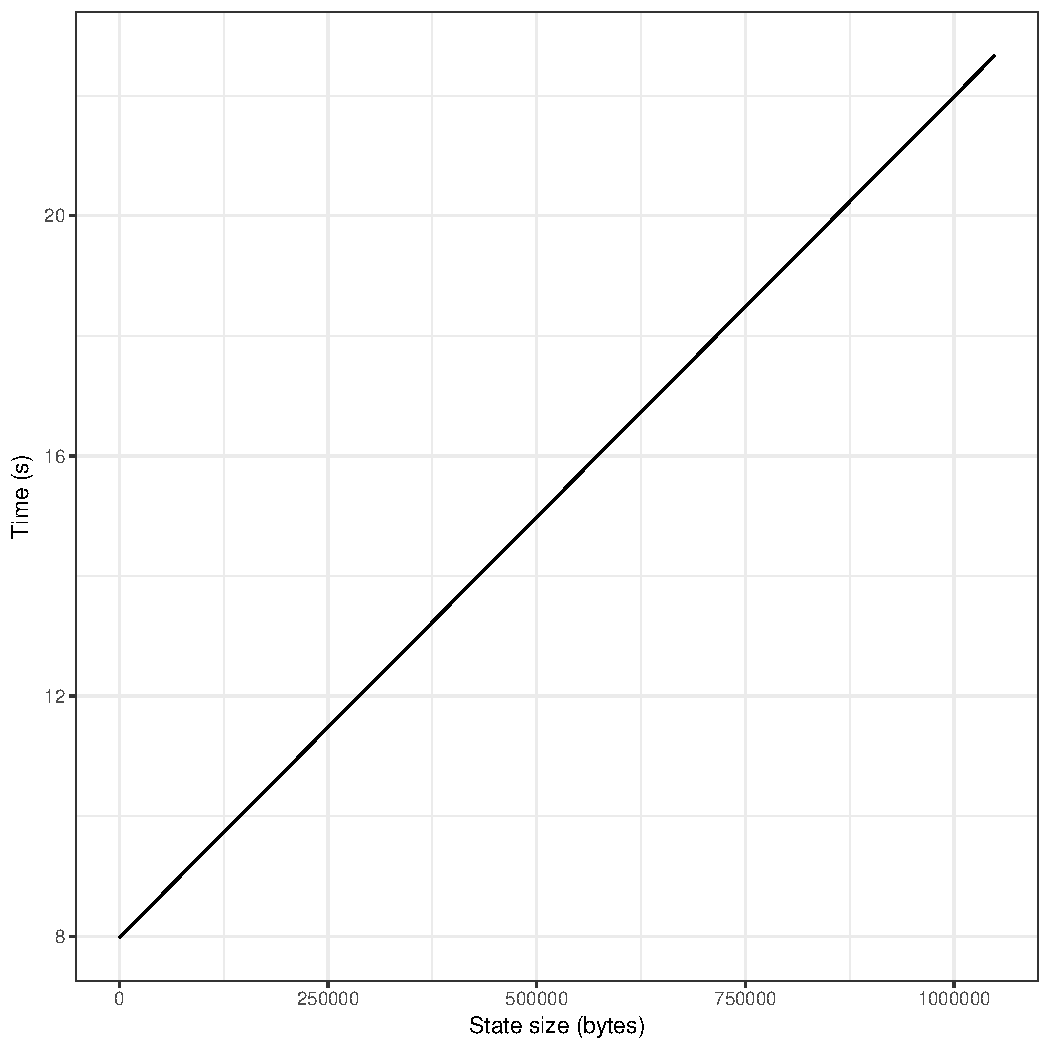
\includegraphics[width=0.9\textwidth]{client-welcome-state-size}
        \caption{Client time to connect as a function of the server state size}\label{fig:client-welcome-state-size}
    \endminipage\hfill
    \minipage{0.32\textwidth}
        \centering
        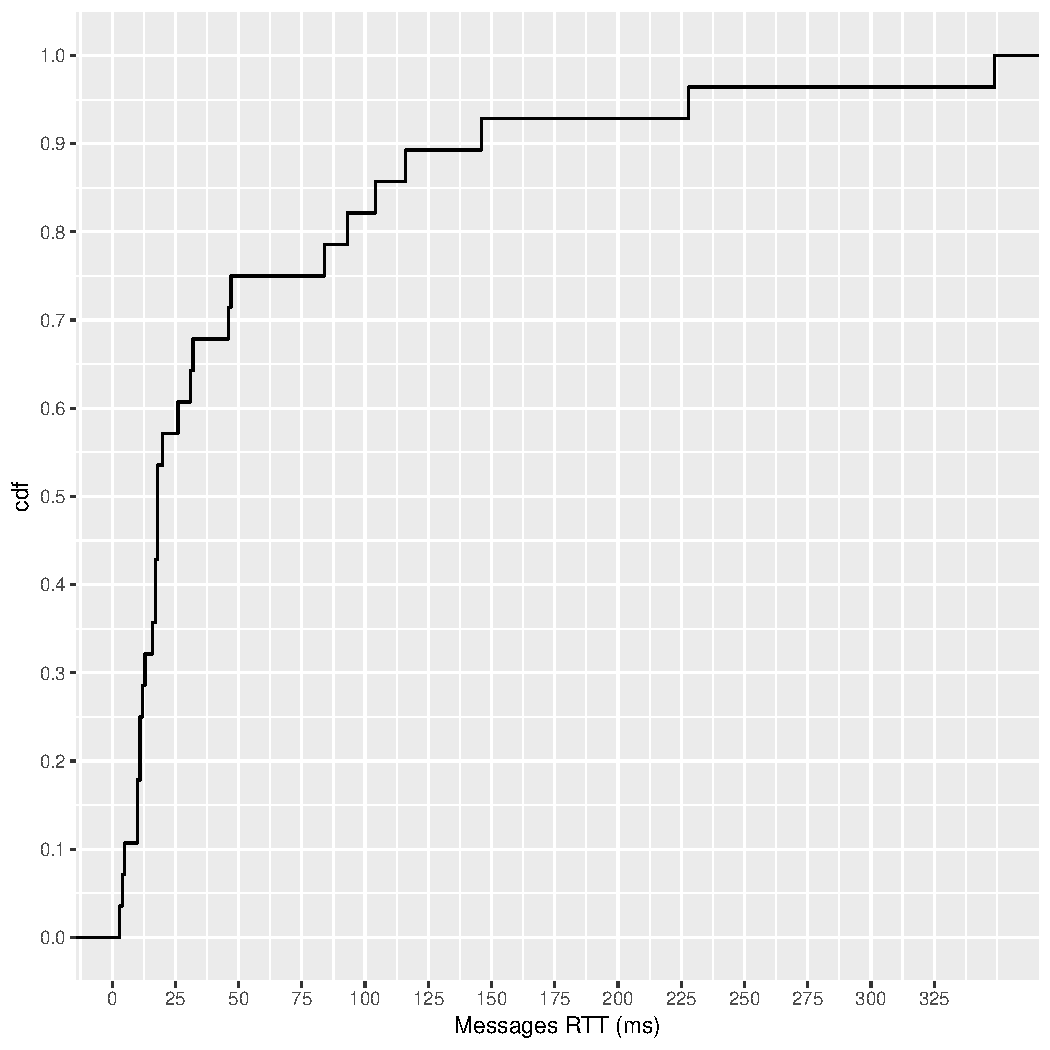
\includegraphics[width=0.9\textwidth]{message-RTT}
        \caption{Operation Round Trip Time}
        \label{fig:message-RTT}
    \endminipage\hfill
    \minipage{0.32\textwidth}%
        \centering
        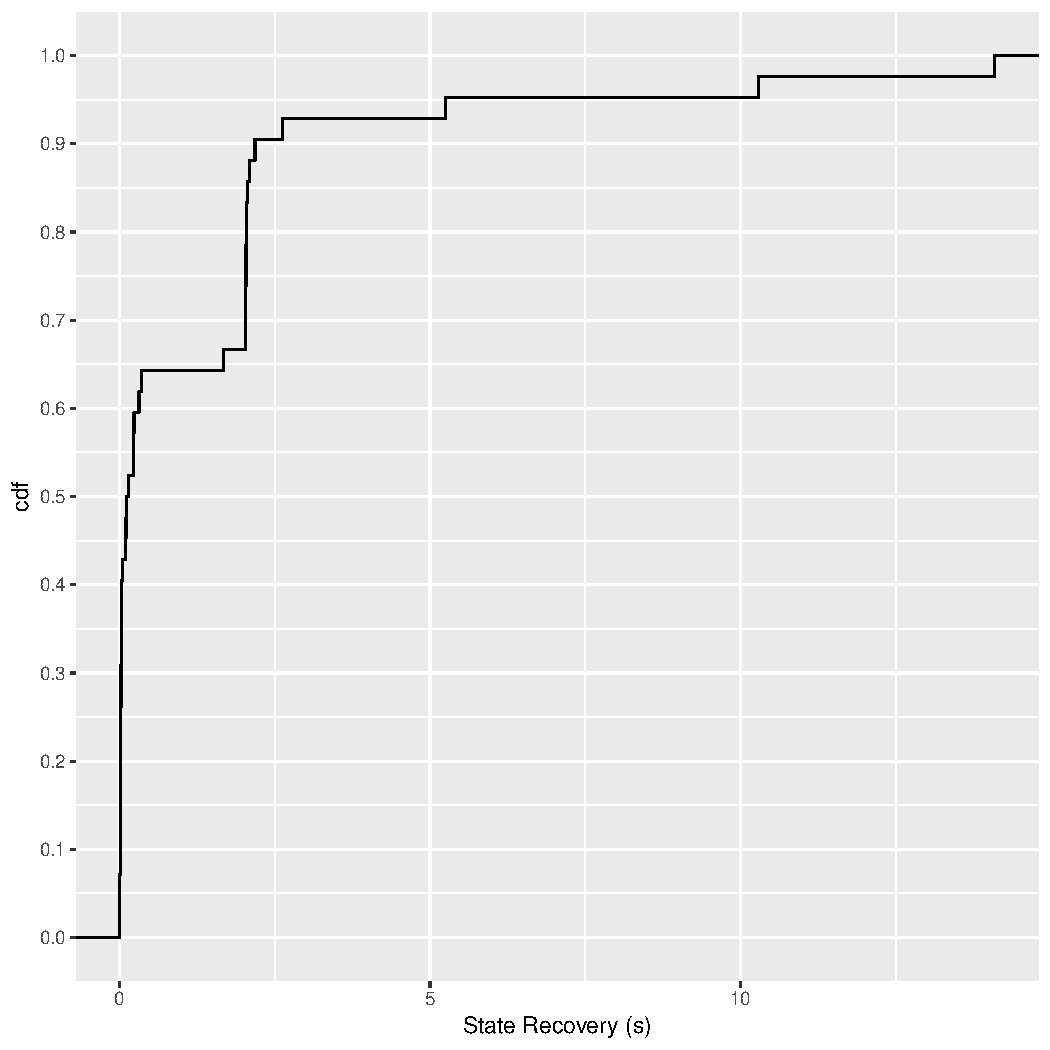
\includegraphics[width=0.9\textwidth]{state-convergence}
        \caption{State convergence - time it takes for all clients to update their state}
        \label{fig:state-convergence}
    \endminipage
\end{figure*}

